\section{交替方向乘子法（ADMM）}
\label{sec:pm-admm}

ALM的子问题比对偶上升的子问题难的地方，在于平方项把各块耦合了。于是要问：当目标由两块组成，能否既保留乘子带来的稳定性，又把两块分开计算？本节的问题形式是
\begin{equation}
 \min_{\bm{x},\bm{z}}\ f(\bm{x})+g(\bm{z})\qquad\text{s.t.}\qquad\bm{A}\bm{x}+\bm{B}\bm{z}=\bm{c},
 \label{eq:pm-admm-problem}
\end{equation}
其中$\bm{x}\in\mathbb{R}^n$，$\bm{z}\in\mathbb{R}^l$，$\bm{A}\in\mathbb{R}^{p\times n}$，$\bm{B}\in\mathbb{R}^{p\times l}$，$\bm{c}\in\mathbb{R}^p$。这里的$g$是第二块目标，不是不等式约束。对应的增广Lagrange函数是
\begin{equation}
 \mathcal{L}_\rho(\bm{x},\bm{z},\bm{\nu})=f(\bm{x})+g(\bm{z})+\langle\bm{\nu},\bm{A}\bm{x}+\bm{B}\bm{z}-\bm{c}\rangle+\frac\rho2\lVert\bm{A}\bm{x}+\bm{B}\bm{z}-\bm{c}\rVert_2^2 .
 \label{eq:pm-admm-al}
\end{equation}

\paragraph{平方项破坏了可分性}
对偶分解能并行，靠的是Lagrange函数按块可分。增广函数的平方项里有交叉项$\rho\langle\bm{A}\bm{x},\bm{B}\bm{z}\rangle$，可分性被破坏。ALM只能把$(\bm{x},\bm{z})$联合起来最小化，即使$f$和$g$各自都很简单。

\term{交替方向乘子法}（alternating direction method of multipliers，ADMM）的想法是：不把子问题解到最优，只把$\bm{x}$和$\bm{z}$各自更新一次，然后立即更新乘子。

这个想法要付代价。用二元例说明，把它看成$f(x)=\tfrac12x^2$，$g(z)=\tfrac32z^2$，$x+z=4$，$\rho=1.5$，$\nu=0$。联合最小化$\mathcal{L}_\rho$得到式~\eqref{eq:pm-running-al-solution}，即$(x,z)=(2,\tfrac23)$。

从$(0,0)$开始交替一次：先固定$z=0$，对$x$最小化，$x=\tfrac{\rho\cdot4}{1+\rho}=2.4$；再固定$x=2.4$，对$z$最小化，$z=\tfrac{\rho(4-2.4)}{3+\rho}=\tfrac{8}{15}$。结果是$(2.4,\tfrac{8}{15})$，与联合解$(2,\tfrac23)$不同。

图~\ref{fig:pm-admm-sweep}(a)画出了这两步：黄色折线先水平走，再竖直走，两步都只顾自己的方向，没有到达碗底。一次交替扫过两块，不等于把子问题解到最优，所以不能把ALM的结论直接搬过来。(b)是多轮的路径，ADMM走的是折线，ALM走的是直线，两者最后都到达红点。

\begin{BookInlineFigure}
  \centering
  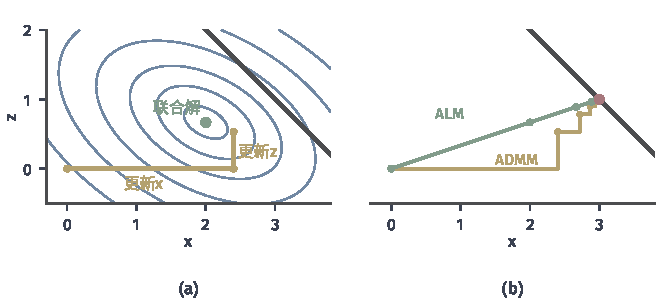
\includegraphics[width=112mm]{figures/05-optimization/06-constrained-optimization/matplotlib/pm-admm-sweep/figure.pdf}
  \caption{二元例上ADMM的两块交替更新，$\rho=1.5$。深灰直线是约束。(a)蓝线是$\nu=0$时增广函数的等高线，绿点是联合最小点$(2,\tfrac23)$，黄色折线是从原点出发的一次交替，停在$(2.4,\tfrac{8}{15})$。(b)绿线是ALM每轮的联合解，黄线是ADMM的折线路径，红点是解$(3,1)$。}
  \label{fig:pm-admm-sweep}
\end{BookInlineFigure}

\subsection{两块交替更新}
\label{sec:pm-admm-update}

\paragraph{主要思想}
每轮按固定的顺序做三步，后一步使用前一步刚得到的结果，如图~\ref{fig:pm-admm-flow}所示：
\begin{equation}
 \begin{aligned}
 \bm{x}^{(t+1)}&\in\argmin_{\bm{x}}\mathcal{L}_\rho(\bm{x},\bm{z}^{(t)},\bm{\nu}^{(t)}),\\
 \bm{z}^{(t+1)}&\in\argmin_{\bm{z}}\mathcal{L}_\rho(\bm{x}^{(t+1)},\bm{z},\bm{\nu}^{(t)}),\\
 \bm{\nu}^{(t+1)}&=\bm{\nu}^{(t)}+\rho\bigl(\bm{A}\bm{x}^{(t+1)}+\bm{B}\bm{z}^{(t+1)}-\bm{c}\bigr).
 \end{aligned}
 \label{eq:pm-admm}
\end{equation}

\begin{BookInlineFigure}
  \centering
  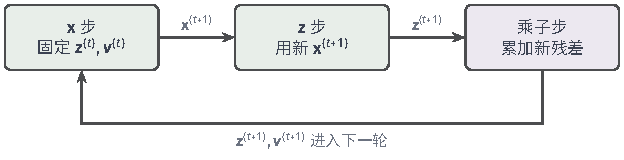
\includegraphics[width=105mm]{figures/05-optimization/06-constrained-optimization/tikz/pm-admm-flow/figure.pdf}
  \caption{ADMM一轮的三步。绿框是两个原始变量的最小化，后一块使用前一块的新值；紫框按新残差累加乘子。与ALM的区别在于$\bm{x}$和$\bm{z}$不联合求解。}
  \label{fig:pm-admm-flow}
\end{BookInlineFigure}

这和第~\ref{chap:block-optimization}章的分块最小化很像：在固定的目标上逐块求最小。两者的区别在于这里有线性耦合约束，单纯的分块下降可能卡在不是解的点上，ADMM靠乘子一步把约束信息累加进下一轮。

\paragraph{缩放乘子}
把乘子除以$\rho$，公式会简短很多。记残差$\bm{r}=\bm{A}\bm{x}+\bm{B}\bm{z}-\bm{c}$，配方得
\[
 \langle\bm{\nu},\bm{r}\rangle+\frac\rho2\lVert\bm{r}\rVert_2^2=\frac\rho2\lVert\bm{r}+\bm{u}\rVert_2^2-\frac\rho2\lVert\bm{u}\rVert_2^2,\qquad\bm{u}=\frac{\bm{\nu}}{\rho}.
\]

$\bm{u}$称为\term{缩放乘子}（scaled dual variable）。式~\eqref{eq:pm-admm}写成缩放形式是
\begin{equation}
 \begin{aligned}
 \bm{x}^{(t+1)}&\in\argmin_{\bm{x}}\ f(\bm{x})+\frac\rho2\lVert\bm{A}\bm{x}+\bm{B}\bm{z}^{(t)}-\bm{c}+\bm{u}^{(t)}\rVert_2^2,\\
 \bm{z}^{(t+1)}&\in\argmin_{\bm{z}}\ g(\bm{z})+\frac\rho2\lVert\bm{A}\bm{x}^{(t+1)}+\bm{B}\bm{z}-\bm{c}+\bm{u}^{(t)}\rVert_2^2,\\
 \bm{u}^{(t+1)}&=\bm{u}^{(t)}+\bm{A}\bm{x}^{(t+1)}+\bm{B}\bm{z}^{(t+1)}-\bm{c}.
 \end{aligned}
 \label{eq:pm-admm-scaled}
\end{equation}
两种写法完全等价。缩放乘子就是残差的累加和，这是它最直观的含义：$\bm{u}^{(t)}$记录到目前为止累计的残差。

\paragraph{套索问题的拆分}
ADMM的用处是把一个有结构的问题拆成两个容易的问题。第~\ref{chap:nonsmooth-composite-optimization}章的套索问题是
\begin{equation}
 \min_{\bm{x}}\ \frac12\lVert\bm{D}\bm{x}-\bm{y}\rVert_2^2+\gamma\lVert\bm{x}\rVert_1 ,
 \label{eq:pm-lasso}
\end{equation}
其中$\bm{D}\in\mathbb{R}^{N\times n}$，$\gamma>0$。把变量复制一份，让$f$负责最小二乘项$\tfrac12\lVert\bm{D}\bm{x}-\bm{y}\rVert_2^2$，$g$负责$\gamma\lVert\bm{z}\rVert_1$，并加上约束$\bm{x}-\bm{z}=\bm{0}$。这对应$\bm{A}=\bm{I}$，$\bm{B}=-\bm{I}$，$\bm{c}=\bm{0}$。

把$f$代入式~\eqref{eq:pm-admm-scaled}的第一行，这是一个二次子问题，解为
\begin{equation}
 \bm{x}^{(t+1)}=(\bm{D}^\top\bm{D}+\rho\bm{I})^{-1}\bigl(\bm{D}^\top\bm{y}+\rho(\bm{z}^{(t)}-\bm{u}^{(t)})\bigr).
 \label{eq:pm-lasso-x}
\end{equation}
第二行是$\gamma\lVert\bm{z}\rVert_1$加上一个以$\bm{x}^{(t+1)}+\bm{u}^{(t)}$为中心的二次项，按坐标可分，由软阈值给出：
\begin{equation}
 \bm{z}^{(t+1)}=S_{\gamma/\rho}\bigl(\bm{x}^{(t+1)}+\bm{u}^{(t)}\bigr),\qquad
 S_\tau(a)=\operatorname{sign}(a)\max\{\lvert a\rvert-\tau,0\}.
 \label{eq:pm-lasso-z}
\end{equation}
第三行是缩放乘子的累加：
\begin{equation}
 \bm{u}^{(t+1)}=\bm{u}^{(t)}+\bm{x}^{(t+1)}-\bm{z}^{(t+1)}.
 \label{eq:pm-lasso-u}
\end{equation}
二次子问题只含$f$，软阈值只含$g$，这样两部分结构都得到了利用。

\paragraph{计算过程}
用第~\ref{chap:nonsmooth-composite-optimization}章的小例子演示，数据是
\[
 \bm{D}=\begin{pmatrix}1&1\\1&0\\0&1\end{pmatrix},\qquad
 \bm{y}=\begin{pmatrix}3\\2\\-1\end{pmatrix},\qquad
 \gamma=1 .
\]
这个问题的解是$\bm{x}^\star=(2,0)$，由它算出乘子
\[
 \bm{\nu}^\star=\bm{D}^\top(\bm{y}-\bm{D}\bm{x}^\star)=(1,0).
\]

\needspace{6\baselineskip}
\paragraph{变量}
\begin{itemize}
 \item $\bm{x}^{(t)},\bm{z}^{(t)}\in\mathbb{R}^n$：两块原始变量。例中$n=2$。
 \item $\bm{u}^{(t)}\in\mathbb{R}^n$：缩放乘子。
 \item $(\bm{D}^\top\bm{D}+\rho\bm{I})^{-1}$：只需计算一次的矩阵分解。
\end{itemize}

\paragraph{初始化}
取$\bm{z}^{(0)}$、$\bm{u}^{(0)}$和$\rho$。例中$\bm{z}^{(0)}=\bm{u}^{(0)}=\bm{0}$，$\rho=1$，并预先算出
\[
 \bm{D}^\top\bm{y}=\begin{pmatrix}5\\2\end{pmatrix},\qquad
 (\bm{D}^\top\bm{D}+\bm{I})^{-1}=\frac18\begin{pmatrix}3&-1\\-1&3\end{pmatrix}.
\]

\needspace{6\baselineskip}
\paragraph{每轮更新}
\begin{enumerate}
 \item 由式~\eqref{eq:pm-lasso-x}算$\bm{x}^{(t+1)}$。例中第一轮
 \[
  \bm{x}^{(1)}=\frac18\begin{pmatrix}3&-1\\-1&3\end{pmatrix}\begin{pmatrix}5\\2\end{pmatrix}=\begin{pmatrix}1.625\\0.125\end{pmatrix}.
 \]
 \item 由式~\eqref{eq:pm-lasso-z}算$\bm{z}^{(t+1)}$，阈值是$\gamma/\rho=1$。例中第一轮
 \[
  \bm{z}^{(1)}=S_1(1.625,\ 0.125)=(0.625,\ 0).
 \]
 \item 由式~\eqref{eq:pm-lasso-u}累加残差。例中第一轮
 \[
  \bm{u}^{(1)}=(1,\ 0.125).
 \]
\end{enumerate}
第二轮中，式~\eqref{eq:pm-lasso-x}的右端向量是$(4.625,1.875)$，得到
\[
 \bm{x}^{(2)}=(1.5,\ 0.125),\qquad \bm{z}^{(2)}=(1.5,\ 0),\qquad \bm{u}^{(2)}=(1,\ 0.25).
\]
第三轮中，右端向量是$(5.5,1.75)$，得到
\[
 \bm{x}^{(3)}=(1.84375,\,-0.03125),\quad \bm{z}^{(3)}=(1.84375,\,0),\quad \bm{u}^{(3)}=(1,\,0.21875).
\]

结束条件由下一小节的残差给出。例中$\bm{z}^{(t)}$从第一轮起就有第二个分量恰好为零，这是软阈值带来的。而$\bm{x}^{(t)}$的第二个分量不为零，只有极限才为零。继续迭代，$24$轮后两种残差都小于$10^{-6}$，最终得到$\bm{z}\approx(2,0)$，$\bm{u}\approx(1,0)$，与上面的$\bm{x}^\star$和$\bm{\nu}^\star$一致。

\subsection{原始与对偶残差}
\label{sec:pm-admm-residuals}

\paragraph{两类残差的来历}
判断ADMM是否收敛，要回到KKT条件。问题~\eqref{eq:pm-admm-problem}的KKT条件有三条：
\begin{equation}
 \bm{A}\bm{x}^\star+\bm{B}\bm{z}^\star=\bm{c},\qquad
 \bm{0}\in\partial f(\bm{x}^\star)+\bm{A}^\top\bm{\nu}^\star,\qquad
 \bm{0}\in\partial g(\bm{z}^\star)+\bm{B}^\top\bm{\nu}^\star .
 \label{eq:pm-admm-kkt}
\end{equation}
第一条对应\term{原始残差}（primal residual）：
\begin{equation}
 \bm{r}^{(t+1)}=\bm{A}\bm{x}^{(t+1)}+\bm{B}\bm{z}^{(t+1)}-\bm{c}.
 \label{eq:pm-admm-primal-residual}
\end{equation}
它度量约束违规。

后两条要看子问题的最优性条件。$\bm{z}^{(t+1)}$最小化$\mathcal{L}_\rho(\bm{x}^{(t+1)},\cdot,\bm{\nu}^{(t)})$，所以
\[
 \bm{0}\in\partial g(\bm{z}^{(t+1)})+\bm{B}^\top\bm{\nu}^{(t)}+\rho\bm{B}^\top\bm{r}^{(t+1)}=\partial g(\bm{z}^{(t+1)})+\bm{B}^\top\bm{\nu}^{(t+1)}.
\]
第三条KKT条件每一轮都自动成立。这也说明了乘子步长取成$\rho$的原因，和式~\eqref{eq:pm-al-gradient-identity}是同一个道理。

$\bm{x}^{(t+1)}$的最优性条件里，用的是旧的$\bm{z}^{(t)}$：
\[
 \bm{0}\in\partial f(\bm{x}^{(t+1)})+\bm{A}^\top\bm{\nu}^{(t)}+\rho\bm{A}^\top\bigl(\bm{A}\bm{x}^{(t+1)}+\bm{B}\bm{z}^{(t)}-\bm{c}\bigr).
\]
用乘子更新式把$\bm{\nu}^{(t)}$换成$\bm{\nu}^{(t+1)}$，整理得到
\begin{equation}
 \rho\bm{A}^\top\bm{B}(\bm{z}^{(t+1)}-\bm{z}^{(t)})\in\partial f(\bm{x}^{(t+1)})+\bm{A}^\top\bm{\nu}^{(t+1)}.
 \label{eq:pm-admm-x-optimality}
\end{equation}
左边的向量就是第二条KKT条件还差的部分，这是\term{对偶残差}（dual residual）：
\begin{equation}
 \bm{s}^{(t+1)}=\rho\bm{A}^\top\bm{B}(\bm{z}^{(t+1)}-\bm{z}^{(t)}).
 \label{eq:pm-admm-dual-residual}
\end{equation}
对偶残差的来源，是$\bm{x}$更新时用了$\bm{z}$的旧值。如果$\bm{x},\bm{z}$是联合求解的，它就恒为零，这正是ALM没有这一项的原因。

例中$\bm{A}=\bm{I}$，$\bm{B}=-\bm{I}$，所以
\[
 \lVert\bm{r}^{(t)}\rVert_2=\lVert\bm{x}^{(t)}-\bm{z}^{(t)}\rVert_2,\qquad
 \lVert\bm{s}^{(t)}\rVert_2=\rho\lVert\bm{z}^{(t)}-\bm{z}^{(t-1)}\rVert_2 .
\]
上面三轮的数值是
\[
 \lVert\bm{r}^{(1)}\rVert_2\approx1.008,\qquad\lVert\bm{r}^{(2)}\rVert_2=0.125,\qquad\lVert\bm{r}^{(3)}\rVert_2\approx0.031,
\]
\[
 \lVert\bm{s}^{(1)}\rVert_2=0.625,\qquad\lVert\bm{s}^{(2)}\rVert_2=0.875,\qquad\lVert\bm{s}^{(3)}\rVert_2\approx0.344 .
\]
可见两个残差并不同步，第二轮原始残差下降，对偶残差反而上升。只看其中一个会误判。图~\ref{fig:pm-admm-lasso}(a)是完整的残差曲线。

\paragraph{停止准则}
两个残差都小才算结束。残差的量级依赖数据的量级，所以常用绝对容差$\varepsilon_{\mathrm{abs}}$和相对容差$\varepsilon_{\mathrm{rel}}$的组合：
\begin{equation}
 \begin{aligned}
 \lVert\bm{r}^{(t)}\rVert_2&\leq\sqrt{p}\,\varepsilon_{\mathrm{abs}}+\varepsilon_{\mathrm{rel}}\max\bigl\{\lVert\bm{A}\bm{x}^{(t)}\rVert_2,\lVert\bm{B}\bm{z}^{(t)}\rVert_2,\lVert\bm{c}\rVert_2\bigr\},\\
 \lVert\bm{s}^{(t)}\rVert_2&\leq\sqrt{n}\,\varepsilon_{\mathrm{abs}}+\varepsilon_{\mathrm{rel}}\lVert\bm{A}^\top\bm{\nu}^{(t)}\rVert_2 .
 \end{aligned}
 \label{eq:pm-admm-stopping}
\end{equation}
绝对容差防止目标为零附近时相对准则失效，$\sqrt{p}$和$\sqrt{n}$让绝对容差按每个分量计。

\paragraph{罚参数的影响与调整}
$\rho$在两个残差之间做权衡。$\rho$大，约束被更用力地压住，原始残差小；可$\bm{s}$正比于$\rho$，对偶残差变大。$\rho$小时情况相反。图~\ref{fig:pm-admm-lasso}(b)是轮数随$\rho$变化的曲线，有一个相当宽的最佳区间，两端都很慢。

一种常见的启发式规则是让两个残差保持同一量级：
\begin{equation}
 \rho^{(t+1)}=
 \begin{cases}
 2\rho^{(t)}, & \lVert\bm{r}^{(t)}\rVert_2>10\lVert\bm{s}^{(t)}\rVert_2,\\
 \rho^{(t)}/2, & \lVert\bm{s}^{(t)}\rVert_2>10\lVert\bm{r}^{(t)}\rVert_2,\\
 \rho^{(t)}, & \text{其他}.
 \end{cases}
 \label{eq:pm-admm-rho}
\end{equation}
这称为\term{残差平衡}（residual balancing）。改变$\rho$时要特别注意缩放乘子。未缩放的$\bm{\nu}$不变，所以$\bm{u}=\bm{\nu}/\rho$必须同步换算：
\begin{equation}
 \bm{u}\leftarrow\frac{\rho^{(t)}}{\rho^{(t+1)}}\bm{u}.
 \label{eq:pm-admm-rescale}
\end{equation}
忘记换算，相当于悄悄改变了乘子，迭代会被打乱。此外，$\rho$变化后需要重新分解矩阵，下面的收敛定理也只对固定的$\rho$成立，实际中常在迭代若干轮后固定$\rho$。

\begin{BookInlineFigure}
  \centering
  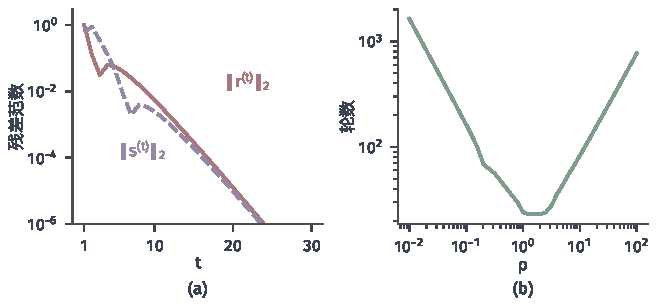
\includegraphics[width=112mm]{figures/05-optimization/06-constrained-optimization/matplotlib/pm-admm-lasso/figure.pdf}
  \caption{小例子上的ADMM。(a)半对数坐标，$\rho=1$，红线是原始残差，紫色虚线是对偶残差。(b)双对数坐标，两个残差都小于$10^{-6}$所需的轮数随$\rho$的变化。两端都慢，中间有一段较宽的平坦区域。}
  \label{fig:pm-admm-lasso}
\end{BookInlineFigure}

\subsection{收敛与实现}
\label{sec:pm-admm-convergence}

\paragraph{收敛定理}
ADMM的步子不是ALM的精确子问题，上一节的定理不能直接用，需要一个专门的证明。证明的想法是构造一个Lyapunov函数，它把乘子误差和$\bm{z}$的误差放在一起，每一轮都下降。

\begin{theorem}[两块ADMM的收敛]
\label{thm:pm-admm-convergence}
设$f,g$是适当、闭的凸函数，固定$\rho>0$，式~\eqref{eq:pm-admm}的两个子问题的最小点存在并精确求解。设$\mathcal{L}_0$有鞍点$(\bm{x}^\star,\bm{z}^\star,\bm{\nu}^\star)$，记$p^\star=f(\bm{x}^\star)+g(\bm{z}^\star)$，$p^{(t)}=f(\bm{x}^{(t)})+g(\bm{z}^{(t)})$，并记
\begin{equation}
 V^{(t)}=\frac1\rho\lVert\bm{\nu}^{(t)}-\bm{\nu}^\star\rVert_2^2+\rho\lVert\bm{B}(\bm{z}^{(t)}-\bm{z}^\star)\rVert_2^2 .
 \label{eq:pm-admm-lyapunov}
\end{equation}
则$t\geq1$时
\begin{equation}
 V^{(t+1)}\leq V^{(t)}-\rho\lVert\bm{r}^{(t+1)}\rVert_2^2-\rho\lVert\bm{B}(\bm{z}^{(t+1)}-\bm{z}^{(t)})\rVert_2^2 ,
 \label{eq:pm-admm-descent}
\end{equation}
并且$\bm{r}^{(t)}\to\bm{0}$，$\bm{s}^{(t)}\to\bm{0}$，$p^{(t)}\to p^\star$。若$\bm{A},\bm{B}$还列满秩，则$\bm{x}^{(t)},\bm{z}^{(t)},\bm{\nu}^{(t)}$都收敛，其极限构成一个鞍点。
\end{theorem}

\begin{proof}
记$\bm{r}=\bm{r}^{(t+1)}$，$\bm{w}=\bm{B}(\bm{z}^{(t+1)}-\bm{z}^{(t)})$。证明分四步。

第一步，用鞍点给出一侧不等式。鞍点满足
\[
 \mathcal{L}_0(\bm{x}^\star,\bm{z}^\star,\bm{\nu}^\star)\leq\mathcal{L}_0(\bm{x}^{(t+1)},\bm{z}^{(t+1)},\bm{\nu}^\star),
\]
再用$\bm{A}\bm{x}^\star+\bm{B}\bm{z}^\star=\bm{c}$，于是
\begin{equation}
 p^\star-p^{(t+1)}\leq\langle\bm{\nu}^\star,\bm{r}\rangle .
 \label{eq:pm-admm-proof-a}
\end{equation}

第二步，用子问题的最优性给出另一侧不等式。上一小节已经推导，$\bm{x}^{(t+1)}$最小化凸函数$f(\bm{x})+\langle\bm{\nu}^{(t+1)}-\rho\bm{w},\bm{A}\bm{x}\rangle$，$\bm{z}^{(t+1)}$最小化凸函数$g(\bm{z})+\langle\bm{\nu}^{(t+1)},\bm{B}\bm{z}\rangle$。分别在$\bm{x}^\star$、$\bm{z}^\star$处比较，得到
\[
 f(\bm{x}^{(t+1)})+\langle\bm{\nu}^{(t+1)}-\rho\bm{w},\bm{A}\bm{x}^{(t+1)}\rangle\leq f(\bm{x}^\star)+\langle\bm{\nu}^{(t+1)}-\rho\bm{w},\bm{A}\bm{x}^\star\rangle,
\]
\[
 g(\bm{z}^{(t+1)})+\langle\bm{\nu}^{(t+1)},\bm{B}\bm{z}^{(t+1)}\rangle\leq g(\bm{z}^\star)+\langle\bm{\nu}^{(t+1)},\bm{B}\bm{z}^\star\rangle .
\]
两式相加。由$\bm{A}\bm{x}^\star+\bm{B}\bm{z}^\star=\bm{c}$，有
\[
 \bm{A}(\bm{x}^{(t+1)}-\bm{x}^\star)+\bm{B}(\bm{z}^{(t+1)}-\bm{z}^\star)=\bm{r},
\]
所以含$\bm{\nu}^{(t+1)}$的项合并成$\langle\bm{\nu}^{(t+1)},\bm{r}\rangle$。再把$\bm{A}(\bm{x}^{(t+1)}-\bm{x}^\star)$换成$\bm{r}-\bm{B}(\bm{z}^{(t+1)}-\bm{z}^\star)$，得到
\begin{equation}
 p^{(t+1)}-p^\star\leq-\langle\bm{\nu}^{(t+1)},\bm{r}\rangle+\rho\langle\bm{w},\bm{r}-\bm{B}(\bm{z}^{(t+1)}-\bm{z}^\star)\rangle .
 \label{eq:pm-admm-proof-b}
\end{equation}

第三步，推导下降不等式。式~\eqref{eq:pm-admm-proof-a}与式~\eqref{eq:pm-admm-proof-b}相加，左边为零，两边乘$2$并移项，得到
\[
 2\langle\bm{\nu}^{(t+1)}-\bm{\nu}^\star,\bm{r}\rangle-2\rho\langle\bm{w},\bm{r}\rangle+2\rho\langle\bm{w},\bm{B}(\bm{z}^{(t+1)}-\bm{z}^\star)\rangle\leq0 .
\]

第一项用$\bm{\nu}^{(t+1)}=\bm{\nu}^{(t)}+\rho\bm{r}$改写，按乘子距离的平方差展开：
\[
 2\langle\bm{\nu}^{(t+1)}-\bm{\nu}^\star,\bm{r}\rangle
 =\frac1\rho\Bigl(\lVert\bm{\nu}^{(t+1)}-\bm{\nu}^\star\rVert_2^2-\lVert\bm{\nu}^{(t)}-\bm{\nu}^\star\rVert_2^2\Bigr)+\rho\lVert\bm{r}\rVert_2^2 .
\]
第三项要用下面的恒等式：
\[
 2\langle\bm{a}-\bm{b},\bm{a}\rangle=\lVert\bm{a}\rVert_2^2-\lVert\bm{b}\rVert_2^2+\lVert\bm{a}-\bm{b}\rVert_2^2 .
\]
取$\bm{a}=\bm{B}(\bm{z}^{(t+1)}-\bm{z}^\star)$，$\bm{b}=\bm{B}(\bm{z}^{(t)}-\bm{z}^\star)$，此时$\bm{a}-\bm{b}=\bm{w}$，于是
\[
 2\rho\langle\bm{w},\bm{a}\rangle=\rho\lVert\bm{a}\rVert_2^2-\rho\lVert\bm{b}\rVert_2^2+\rho\lVert\bm{w}\rVert_2^2 .
\]
把这两式代回，合并成
\[
 V^{(t+1)}-V^{(t)}+\rho\lVert\bm{r}\rVert_2^2+\rho\lVert\bm{w}\rVert_2^2-2\rho\langle\bm{w},\bm{r}\rangle\leq0 .
\]

只差$\langle\bm{w},\bm{r}\rangle$的符号。设$t\geq1$，$\bm{z}^{(t)}$也是上一轮的子问题解，最小化$g(\bm{z})+\langle\bm{\nu}^{(t)},\bm{B}\bm{z}\rangle$。把它和$\bm{z}^{(t+1)}$的最优性互相比较，
\[
 g(\bm{z}^{(t+1)})+\langle\bm{\nu}^{(t+1)},\bm{B}\bm{z}^{(t+1)}\rangle\leq g(\bm{z}^{(t)})+\langle\bm{\nu}^{(t+1)},\bm{B}\bm{z}^{(t)}\rangle,
\]
\[
 g(\bm{z}^{(t)})+\langle\bm{\nu}^{(t)},\bm{B}\bm{z}^{(t)}\rangle\leq g(\bm{z}^{(t+1)})+\langle\bm{\nu}^{(t)},\bm{B}\bm{z}^{(t+1)}\rangle .
\]
相加后，$g$的项全部消去，剩下
\[
 \langle\bm{\nu}^{(t+1)}-\bm{\nu}^{(t)},\bm{w}\rangle\leq0 ,
\]
也就是$\rho\langle\bm{r},\bm{w}\rangle\leq0$。于是$-2\rho\langle\bm{w},\bm{r}\rangle\geq0$，舍去后即得式~\eqref{eq:pm-admm-descent}。

第四步，取极限。对式~\eqref{eq:pm-admm-descent}求和，$\sum_t\lVert\bm{r}^{(t)}\rVert_2^2$和$\sum_t\lVert\bm{w}\rVert_2^2$都有限，所以$\bm{r}^{(t)}\to\bm{0}$，$\bm{B}(\bm{z}^{(t+1)}-\bm{z}^{(t)})\to\bm{0}$，进而$\bm{s}^{(t)}\to\bm{0}$。同时$V^{(t)}$有界，所以$\bm{\nu}^{(t)}$和$\bm{B}\bm{z}^{(t)}$都有界。式~\eqref{eq:pm-admm-proof-b}的右边因此趋于零，式~\eqref{eq:pm-admm-proof-a}的右边也趋于零，夹逼得$p^{(t)}\to p^\star$。

最后设$\bm{A},\bm{B}$列满秩。$\bm{B}\bm{z}^{(t)}$有界推出$\bm{z}^{(t)}$有界，再由$\bm{r}^{(t)}\to\bm{0}$推出$\bm{A}\bm{x}^{(t)}$有界，从而$\bm{x}^{(t)}$有界。

取一个收敛子列，极限记为$(\hat{\bm{x}},\hat{\bm{z}},\hat{\bm{\nu}})$。在$\bm{r}=\bm{0}$、最优性包含式~\eqref{eq:pm-admm-x-optimality}和$\bm{z}$的最优性条件里取极限（闭凸函数的次微分图像是闭的），可知极限满足KKT条件~\eqref{eq:pm-admm-kkt}，所以它是鞍点。

式~\eqref{eq:pm-admm-descent}对任意鞍点成立。取这个鞍点作为比较点，$V^{(t)}$单调不增且沿子列趋于零，所以整列趋于零。再由列满秩，$\bm{x}^{(t)},\bm{z}^{(t)},\bm{\nu}^{(t)}$整列收敛。
\end{proof}

定理的各部分有不同的强度。残差和目标值的收敛只需要鞍点存在。在没有列满秩的一般情形下，$\bm{\nu}^{(t)}$本身也收敛到某个最优乘子，这个结论可以从ADMM与Douglas--Rachford分裂的等价关系得到，证明需要算子分裂的不动点理论，篇幅较长，这里只使用结论。

原始变量的整列收敛则确实需要额外条件。$\bm{A}$不是列满秩时，$\bm{x}$可以在$\operatorname{null}(\bm{A})$方向上不确定，子问题的解都不唯一，序列没有理由收敛。

\paragraph{实现中的计算}
ADMM每轮的代价取决于两个子问题。套索的例子中，$\bm{x}$更新要解以$\bm{D}^\top\bm{D}+\rho\bm{I}$为系数的线性系统，$\rho$固定时这个矩阵只需分解一次。一次Cholesky分解约需$O(n^3)$次运算，此后每轮只需$O(n^2)$次前代和回代。

当$N\ll n$时，用矩阵求逆引理转化为$N\times N$的系统，分解成本降为$O(N^2n)$。$\bm{z}$更新是逐坐标的软阈值，只需$O(n)$。

分布式的场合，$\bm{x}$和$\bm{z}$常放在不同机器上，每轮通信量是一个残差大小的向量。与联合求解的ALM比较，ADMM的单轮代价低，通信轮数多。ADMM的典型行为是前面几十轮到达中等精度，此后缓慢收敛，所以适合中等精度的问题。

\paragraph{子问题的精度}
定理要求子问题精确求解。实际上线性系统用迭代法解，或者子问题本身没有闭式解。凸的情形下，只要各轮的误差可和，收敛结论仍然成立，证明需要把误差项带入上述下降不等式，并做累加估计。内层精度不够时，$\bm{x}$的最优性条件~\eqref{eq:pm-admm-x-optimality}有一个误差项，所以对偶残差$\bm{s}$不再完全反映驻定误差，需要另外监控子问题的残差。

\paragraph{多块与非凸}
从形式上看，把两块推广到三块只是多写一行，但保证不能沿用。有一个三块的反例：
\[
 \min\ 0\qquad\text{s.t.}\qquad\bm{a}_1x_1+\bm{a}_2x_2+\bm{a}_3x_3=\bm{0},
\]
其中$\bm{a}_1=(1,1,1)$，$\bm{a}_2=(1,1,2)$，$\bm{a}_3=(1,2,2)$。系数矩阵可逆，唯一解是原点，目标是常数$0$。按三块逐块更新，$\rho=1$。数值计算给出这个线性迭代矩阵的谱半径约为$1.028>1$，所以序列从几乎任何初值出发都发散。

图~\ref{fig:pm-admm-threeblock}中，红线是三块更新的残差，一直增长；绿线把后两块合并成一块，按两块ADMM更新，残差下降。这个例子的目标恒为零，每个子问题都精确可解，失败的原因只在更新的结构上。

\begin{BookInlineFigure}
  \centering
  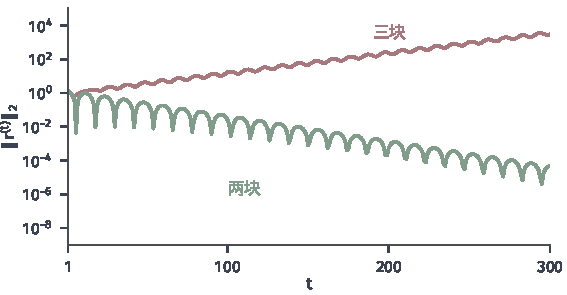
\includegraphics[width=96mm]{figures/05-optimization/06-constrained-optimization/matplotlib/pm-admm-threeblock/figure.pdf}
  \caption{同一个线性系统上的三块与两块ADMM，$\rho=1$，半对数坐标，初值$\bm{x}^{(0)}=(1,1,1)$，乘子初值为零。红线是逐块更新三块的残差，发散；绿线把后两块合并成一块，收敛。}
  \label{fig:pm-admm-threeblock}
\end{BookInlineFigure}

非凸问题上的ADMM使用很广，但一般只能保证在额外的结构条件下收敛到驻点，有时需要$\rho$足够大，有时根本不收敛。一个非凸改写在形式上和ADMM相同，并不意味着上面的定理适用，每种情形都需要重新分析。结束时仍然要回到原约束和最优性条件上去检查。
